% ===========================================================================
% 基于 DeepONet 的 EAST 汤姆逊散射剖面拟合神经网络方法
% 中文阅读检查版 —— 与 manuscript_fed.tex（FED 投稿版，2026-09-09 修订）同步
% 说明：本文件仅供中文阅读检查；投稿以英文版 manuscript_fed.tex 为准。
% ===========================================================================

\documentclass[a4paper,12pt]{ctexart}

% ---- Packages ----
\usepackage{amsmath,amssymb}
\usepackage{graphicx}
\usepackage{booktabs}
\usepackage{multirow}
\usepackage{hyperref}
\usepackage[margin=2.5cm]{geometry}
\usepackage{caption}
\usepackage{subcaption}
\usepackage{enumitem}
\usepackage{microtype}

\sloppy
\hyphenpenalty=1000
\tolerance=2000
\emergencystretch=2em

% ---- Metadata ----
\title{基于 DeepONet 的 EAST 托卡马克汤姆逊散射剖面拟合方法}

\author{%
胡程一璟$^{1,2,3}$，臧庆$^{3,\ast}$\thanks{通讯作者：臧庆（zangq@ipp.ac.cn）。} \\[4pt]
$^1$ 安徽理工大学，淮南 232001 \\
$^2$ 合肥综合性国家科学中心能源研究院 \\
（安徽省能源实验室），合肥 230031 \\
$^3$ 中国科学院等离子体物理研究所，合肥 230031
}

\date{\today}

\begin{document}
\maketitle

\begin{abstract}
\small
EAST 托卡马克的汤姆逊散射（TS）诊断在 20--30 个空间通道上提供电子温度（$T_e$）和密度（$n_e$）的离散测量；重建连续剖面是输运分析和平衡重建的前提。目前广泛使用的改进型双曲正切（mtanh）方法依赖诊断特定的代码分支和手工调整参数，难以规模化处理每年数千炮放电。本文提出一种基于 DeepONet 的神经网络，将七步 mtanh 流程压缩为单次 14 ms 前向传播，在来自 161 炮 EAST 放电的（散点, mtanh 拟合剖面）数据对上训练。共对比五种架构：ProfileNet、BiLSTM、Transformer 和 CNN-DeepONet 共享同一 CoordDecoder 主干网络和物理约束损失函数，纯 CNN-1D 作为控制组。在 68 个未见测试剖面（5 炮、24 个时间点）上，覆盖 L 模至强 H 模条件（$T_e = 0.2$--$7.2$ keV），网络相对 mtanh 基线的平均绝对误差为 $T_e = 0.34$--$0.51$ keV、$n_e = 0.06$--$0.11 \times 10^{19}$ m$^{-3}$、$T_i = 0.07$--$0.14$ keV。

消融实验表明，移除物理约束后 ProfileNet（$-11.8\%$）和 Transformer（$-8.7\%$）略有改善，而 CNN-1D（$+25.8\%$）和 LSTM（$+30.6\%$）退化。分支--主干点积结构将输出限定为光滑基函数的线性组合——对池化和注意力类编码器，光滑性由结构保证而非靠惩罚项；循环分支则仍需显式约束。受控的 CNN-DeepONet 变体（CNN 编码器配共享主干）消解了编码器/解码器混淆：主干解码器显著改善 $T_i$（0.142 降至 0.082 keV）但对 Te、ne 无益。逐剖面拟合的高斯过程回归基线样本内精度更高，但推理成本是 NN 的 6--10 倍。没有单一架构在所有诊断上最优；本文建议部署诊断匹配的集成模型（CNN-Te + ProfileNet-ne + LSTM-Ti，总推理时间 <50 ms）。
\end{abstract}

\noindent\textbf{关键词}：EAST 托卡马克，汤姆逊散射，剖面拟合，DeepONet，神经网络，物理约束学习

% ===========================================================================
% 1. 引言
% ===========================================================================
\section{引言}

中国科学院等离子体物理研究所（ASIPP）的 EAST（Experimental Advanced Superconducting Tokamak）是全超导托卡马克装置，致力于长脉冲、高性能等离子体运行~\cite{east_overview}。理解动理学剖面的空间结构——电子温度 $T_e(\rho)$、电子密度 $n_e(\rho)$ 和离子温度 $T_i(\rho)$ 随归一化小半径 $\rho$ 的分布——对输运分析和平衡重建至关重要。EAST 的汤姆逊散射（TS）诊断在约 20--30 个空间通道上测量 $T_e$ 和 $n_e$~\cite{east_ts,east_tvts}，辅以更高分辨率的反射计（Refl）$n_e$ 测量和 X 射线晶体谱仪（TXCS）$T_i$ 测量。这些离散散点必须重建为连续剖面，才能用于 ONETWO~\cite{onetwo} 或 TRANSP 等程序。

EAST 上剖面拟合的标准方法是改进型双曲正切（mtanh）函数~\cite{mtanh_groebner}：将剖面划分为芯部样条区（$\rho < 0.85$）和台基 mtanh 区（$\rho > 0.85$），通过平滑过渡连接。该方法物理动机明确、经验验证充分，但实践中存在真实局限。整个流程是七步链条（IQR 异常值剔除、芯部样条拟合、台基 mtanh 优化、平滑过渡、左边界修正），实现为六条诊断特定的代码分支。每条分支都带有手工调整参数（台基位置、IQR 阈值、样条节点），在异常放电上可能失效；每次拟合都需要人工目视检查；台基最小二乘优化对初值敏感。这些问题限制了其对 EAST 每年数千炮放电的可扩展性。

机器学习已进入聚变诊断领域：高斯过程回归用于剖面拟合~\cite{gpr_profiles,gpr_review}，贝叶斯集成数据分析~\cite{ida_east}，神经网络用于 TS 时间超分辨~\cite{diag2diag}，以及基于 CNN 的密度剖面重建~\cite{lan_cnn_east}。深度算子网络（DeepONet）~\cite{deeponet} 是专门学习函数空间之间映射的架构，将算子 $G: u \mapsto G(u)$ 分离为编码输入函数的分支网络和编码输出域的主干网络~\cite{physics_informed_deeponet,pinn_review}。分支-主干形式具有本文始终依赖的一个性质：输出 $\hat{y}(\rho) = \sum b_k \cdot t_k(\rho)$ 恒为光滑基函数的线性组合。非物理振荡被结构性地排除，本文将该架构本身视为剖面拟合的\textit{结构性正则化}。

本文提出一种基于 DeepONet 的神经网络，将七步 mtanh 流程替换为单次约 14 ms 前向传播。共对比五种架构——四种（ProfileNet（SetEncoder）、BiLSTM、Transformer 和 CNN-DeepONet）共享同一 CoordDecoder 和物理约束损失，纯 CNN-1D 作为不使用分支-主干结构的控制组——从而实现对架构归纳偏置的受控研究。本文贡献包括：（1）据我们所知，首次将 DeepONet 应用于 EAST TS 剖面拟合；（2）统一条件下的五架构系统对比；（3）受控的 CNN-DeepONet 变体消解编码器/解码器混淆，证明共享主干解码器对稀疏诊断（Ti）有益、对密集诊断（Te、ne）无益；（4）消融实验证明分支-主干结构对静态编码器本身具有正则化作用（移除物理约束后 ProfileNet 和 Transformer 改善 8--12\%，而 CNN-1D 和 LSTM 退化 26--31\%）；（5）发现反映诊断空间采样固有差异的诊断-架构匹配规律；（6）量化下游 LHW 电流驱动影响（平均绝对偏差 22\%，156400 炮；四个 LHW 测试炮合计 28\%），并给出偏差的 $T_e$/$n_e$ 归因分解。简言之，本文的方法学创新在于两个相互交织的思想：将算子学习结构本身当作内置正则化器；以及通过实验设计（共享主干、受控 CNN-DeepONet 变体、统一物理约束损失）使这一论断可被检验而非仅被假定。

% ===========================================================================
% 2. 方法
% ===========================================================================
\section{方法}

\subsection{问题定义}

给定 $N$ 个离散诊断测量点 $\{(\rho_i, y_i)\}_{i=1}^N$，其中 $\rho_i \in [0, 1]$ 为归一化小半径，$y_i$ 为物理量（$T_e$ 单位 eV、$n_e$ 单位 $10^{19}$ m$^{-3}$、$T_i$ 单位 keV），$N$ 随诊断不同通常在 5 到 35 之间。目标是学习映射 $\mathcal{F}$，输出在 $\rho \in [0, 1]$ 上 201 点均匀网格的光滑剖面 $\hat{y}(\rho)$。

mtanh 方法通过显式参数化流程实现 $\mathcal{F}$：IQR 异常值剔除 $\to$ 芯部样条拟合 $\to$ 台基 mtanh 参数优化 $\to$ 平滑过渡 $\to$ 左边界修正。相比之下，神经网络方法在（散点, 拟合剖面）对的数据集上通过监督学习隐式学习 $\mathcal{F}$。

\subsection{训练数据}

训练数据来自 EAST 2015--2024 年度放电（161 炮，炮号 60150--149600）。对每个有诊断数据的（炮号, 时间）对，运行标准 mtanh 流程生成 201 点拟合剖面作为训练标签。原始诊断散点——不经过 IQR 清洗——作为神经网络输入。构造散点输入时，无效通道（非有限读数或低于诊断特定有效性阈值的值）被掩码剔除；所有编码器天然接受变长点集，CNN-1D 额外将掩码编码为第二输入通道。

\textbf{H 模/L 模分类}：能量约束因子 $H_{98}$ 从 EAST MDSplus \texttt{energy\_east} 树（$\backslash$H98\_MHD 信号）读取。$H_{98} \geq 0.7$ 的时间点分类为 H 模，$0 < H_{98} < 0.7$ 为 L 模，$H_{98} = 0$ 为未知（数据不可用）。0.7 的阈值位于典型 L 模约束值与标称 H 模水平（$H_{98}(y,2) \approx 1.0$）之间；$H_{98}$ 读数无效的时间点被排除在分模式对比之外。

\textbf{保留的测试集}：为防止数据泄漏，测试集仅由训练炮号范围（60150--149600）之外的 2024 年放电构成；测试数据不参与训练或验证。训练/验证划分比例为 70/15/15。测试集包含 5 炮 2024 年未参与训练的放电（156005、156010、156100、156400、156900），覆盖 L 模至强 H 模条件（$T_e = 0.2$--$7.2$ keV）。另有两次 2024 年放电经检查后被排除：156200 的 EFIT 平衡覆盖仅到 10.6 s，而其 TS 数据在 32--101 s（$\rho$ 映射不可靠）；156900 的最后两个时间点（7.5--8.5 s，放电降相段）的 mtanh 参考剖面变为非物理。测试集概况见表~\ref{tab:testset}。

\begin{table}[htbp]
\centering\footnotesize
\caption{测试集特征。5 炮均来自 2024 年 EAST 实验，完全排除在训练集外。$T_e$ 范围为该炮各时间点 mtanh 拟合芯部 $T_e$ 的取值范围。}
\label{tab:testset}
\resizebox{\textwidth}{!}{%
\begin{tabular}{cccccccc}
\toprule
\textbf{炮号} & \textbf{时间点数} & \textbf{$T_e$ 范围 (keV)} & \textbf{模式 (H/L/未知)} & \textbf{$H_{98}$ 范围} & \textbf{TS} & \textbf{Refl} & \textbf{TXCS} \\
\midrule
156005 & 2 & 2.3--2.4 & 1H / 1L & 0.69--0.96 & \checkmark & \checkmark & \checkmark \\
156010 & 6 & 0.2--2.0 & 6 未知 & 0.0$^*$ & \checkmark & \checkmark & \checkmark \\
156100 & 6 & 1.2--3.3 & 1H / 5L & 0.56--1.10 & \checkmark & \checkmark & \checkmark \\
156400 & 6 & 3.8--7.2 & 6H & 0.85--1.15 & \checkmark & \checkmark & \checkmark \\
156900 & 4 & 0.2--1.1 & 4L & 0.70$^{\dagger}$ & \checkmark & \checkmark & -- \\
\midrule
合计 & 24 & 0.2--7.2 & 8H / 10L / 6 未知 & --- & 24 & 24 & 20 \\
\bottomrule
\end{tabular}%
}
\vspace{4pt}
\footnotesize{$^*$ 炮号 156010：MDSplus 无 $H_{98}$ 数据（返回 0.0），等离子体模式标记为"未知"。$^{\dagger}$ 炮号 156900：$H_{98}$ 信号仅到 2.53 s；所有时间点使用最后一个可用值（0.698），据此分类为 L 模。该炮无 TXCS（$T_i$）数据。}
\end{table}

\subsection{模型架构}

五种架构中的四种共享同一 DeepONet 风格解码器，仅在编码器设计上不同（图~\ref{fig:architecture}）；第五种 CNN-1D 使用纯卷积解码器作为控制组。共享的 \textbf{CoordDecoder}（主干网络）是 MLP(1$\to$128$\to$128, SiLU)，将输出坐标 $\rho$ 映射为基函数 $\mathbf{b}(\rho) \in \mathbb{R}^{128}$。最终输出为：
\begin{equation}
\hat{y}(\rho) = \operatorname{Softplus}\left(\mathbf{z} \cdot \mathbf{b}(\rho)\right) = \operatorname{Softplus}\left(\sum_{k=1}^{128} z_k \cdot b_k(\rho)\right)
\label{eq:dotproduct}
\end{equation}
其中 $\mathbf{z} \in \mathbb{R}^{128}$ 是编码器产生的潜在向量。Softplus 激活函数（$\ln(1 + e^x)$）确保预测物理量的正值性。

\begin{figure}[htbp]
\centering
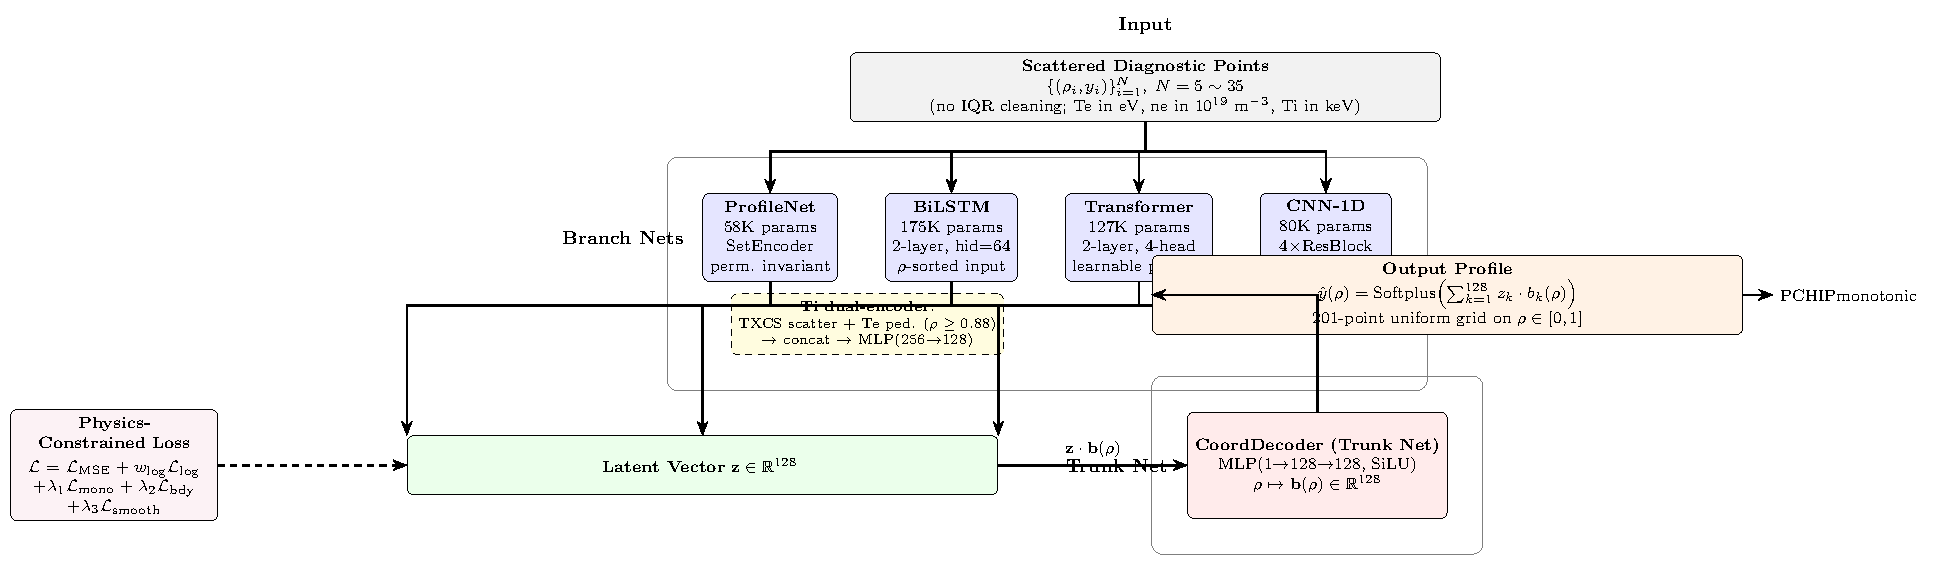
\includegraphics[width=\textwidth]{fig1_architecture.pdf}
\caption{基于 DeepONet 的 TS 剖面拟合架构。四种 DeepONet 编码器变体（分支网络）——ProfileNet、BiLSTM、Transformer 和 CNN-DeepONet——将离散诊断散点编码为潜在向量 $\mathbf{z}$。共享的 CoordDecoder（主干网络）将输出坐标 $\rho$ 映射为光滑基函数 $\mathbf{b}(\rho)$。点积 $\mathbf{z}\cdot\mathbf{b}(\rho)$ 经 Softplus 激活后产生连续剖面 $\hat{y}(\rho)$。第五种架构 CNN-1D 使用纯卷积编解码层、不含分支-主干结构，作为控制组。Ti 模型采用双编码器设计（TXCS 散点 + Te 台基）。训练由物理约束损失监督，结合区域加权 MSE 与单调性、边界和光滑性惩罚项。}
\label{fig:architecture}
\end{figure}

\begin{figure}[htbp]
\centering
\includegraphics[width=0.95\textwidth]{paper_results/figures/fig2_hmode_overlay.png}
\caption{典型 H 模剖面拟合结果：六种方法（mtanh 基线 + 五种 NN 架构）在三个代表性 H 模时间点上对 Te、ne、Ti 三种诊断的对比。}
\label{fig:hmode}
\end{figure}

在图~\ref{fig:hmode} 中，好的拟合可以直接判读：剖面应穿过芯部诊断通道、复现 mtanh 基线的整体形状，更重要的是在 $\rho = 0.85$--$1.0$ 处跟踪陡峭的台基梯度（H 模物理信息集中之处）；剖面应保持光滑、正值、单调，边缘区域无非物理振荡。过度平滑台基或在边缘振荡的架构，在表~\ref{tab:metrics} 的 MAE 指标上相应地更差——该指标量化的正是这些偏差。

\subsubsection{编码器架构}

\textbf{ProfileNet（67K 参数）}：PointNet 风格的 SetEncoder~\cite{pointnet}，对每个散点独立进行 MLP 处理，经最大池化聚合后投影到 $\mathbf{z}$。该架构具有排列不变性——诊断点的顺序不影响输出。

\textbf{LSTM（76K 参数）}：单层双向 LSTM~\cite{lstm}（隐藏维度 64）处理按 $\rho$ 排序的散点，前向和后向最终隐藏状态拼接后投影到 $\mathbf{z}$。BiLSTM 沿 $\rho$ 坐标捕捉径向序列结构。

\textbf{Transformer（136K 参数）}：两层 TransformerEncoder~\cite{transformer}（4 头自注意力，隐藏维度 64），带可学习位置编码，处理排序后的散点。自注意力允许每个诊断通道直接关注任何其他通道，捕捉全局相关性。

\textbf{CNN-DeepONet（79K 参数）}：CNN 编码器——Conv1d 主干、3 个 ResidualBlock1D 和全局最大池化——与 CNN-1D 的编码器一致，但经分支-主干点积接入共享 CoordDecoder。该变体用于消解原对比中的混淆：CNN-1D 在编码器和解码器两端都与其他三个模型不同，其较差表现无法单独归因于任一端。将 CNN 编码器与共享主干配对即可隔离解码器的贡献。

\textbf{CNN-1D（66K 参数，控制组）}：纯 1D ResNet，含 4 个 ResidualBlock1D。\textbf{该架构特意不使用 DeepONet 分支-主干结构。}散点线性插值到 201 点网格，堆叠为 2 通道张量 [values, mask]，经 Conv1d 编解码器和残差连接处理。不使用 BatchNorm。与 CNN-DeepONet 配对，该控制组可隔离分支-主干解码器在其余部分完全相同的 CNN 编码器下的效应。

\subsubsection{Ti 双编码器}

所有架构的 $T_i$ 变体使用双编码器设计：一个编码器处理 TXCS 散点（主输入），另一个处理 $T_e$ 台基数据（$\rho \geq 0.88$）。两个潜在向量拼接后经 MLP(256$\to$128$\to$128) 融合。该设计对标 mtanh 借用 $T_e$ 台基信息约束 $T_i$ 边缘拟合的实践。

\subsection{物理约束损失函数}

训练目标结合区域加权 MSE 与物理启发的辅助项：

\begin{equation}
\mathcal{L} = \mathcal{L}_{\text{MSE}} + w_{\log} \mathcal{L}_{\log} + \lambda_1 \mathcal{L}_{\text{mono}} + \lambda_2 \mathcal{L}_{\text{bdy}} + \lambda_3 \mathcal{L}_{\text{smooth}}
\label{eq:loss}
\end{equation}

\begin{itemize}
    \item $\mathcal{L}_{\text{MSE}}$：区域加权 MSE（芯部 $\rho < 0.85$：3$\times$，台基 $\rho \geq 0.85$：25$\times$），优先保证台基区域的重建精度。
    \item $\mathcal{L}_{\log}$（$w_{\log}=0.1$）：对数空间 MSE，惩罚低值边缘区域中绝对误差虽小但物理意义显著的相对误差。
    \item $\mathcal{L}_{\text{mono}}$（$\lambda_1=0.05$）：$\operatorname{ReLU}(+d\hat{y}/d\rho)$，仅惩罚正导数，即本应随 $\rho$ 单调递减的剖面中出现的局部非单调抬升。不强求全局单调性，只抑制局部非物理抬升。
    \item $\mathcal{L}_{\text{bdy}}$（$\lambda_2=0.05$）：在 $\rho < 0.05$ 区域最小化 $|d\hat{y}/d\rho|$，施加磁轴对称条件 $dT/d\rho|_{\rho=0} = 0$。
    \item $\mathcal{L}_{\text{smooth}}$（$\lambda_3=0.01$）：惩罚大值二阶导数 $|d^2\hat{y}/d\rho^2|$，抑制高频振荡。
\end{itemize}

惩罚权重（$\lambda_1$、$\lambda_2$、$\lambda_3$、$w_{\log}$）在验证集上经验设定，并在所有架构间保持一致以保证可比性；其影响在消融实验（表~\ref{tab:ablation}）中直接检验。

\subsection{训练细节}

所有模型使用 AdamW 优化器（学习率 $10^{-3}$，权重衰减 $10^{-5}$）、余弦退火学习率调度、批次大小 64、最大 500 轮训练和早停机制（耐心值 = 100）。推理后应用 PCHIP（分段三次 Hermite 插值）保形插值，强制严格单调递减和边缘地板值保护。所有报告的指标均在后处理之后的剖面上计算；我们在 Te 测试点上验证过，PCHIP 步骤对散点拟合 MAE 和相对 mtanh 的 MAE 的影响均小于 0.001 keV，即不会实质改变报告数值。推理时间在 CPU 上测量（10 次预热后对完整推理函数计时 200 次，不含模型加载）。

五种架构在单核 CPU 上的推理时间均低于约 20 ms（ProfileNet $\sim$15 ms、LSTM $\sim$14 ms、CNN-1D $\sim$16 ms、CNN-DeepONet $\sim$16 ms、Transformer $\sim$19 ms），既适用于离线批量处理，也满足潜在实时应用需求。作为参照，我们在同一 CPU 上对 24 个测试点计时了 mtanh 流程端到端运行时间：每个 Te 剖面 16--71 ms（中位数 36 ms），$n_e$ 为 16--870 ms（中位数 30 ms；最小二乘收敛缓慢造成长尾），$T_i$ 约 1 ms（其参数化拟合比 NN 更轻）。因此 NN 对 Te 比 mtanh 快 2--3 倍，在 $n_e$ 的慢收敛情形下更快，而对 $T_i$ 的原始时延反而慢于 mtanh。实际收益并非单纯的速度，而是统一性：一次确定性的 14--19 ms 前向传播，无逐例优化器失败模式、无需人工检查。诊断最优集成方案（CNN-based $T_e$ + ProfileNet-based $n_e$ + LSTM-based $T_i$，共 66K+67K+76K 参数）组合推理时间低于 50 ms。

% ===========================================================================
% 3. 结果
% ===========================================================================
\section{结果}

\subsection{拟合精度：五种架构 vs. mtanh}

表~\ref{tab:metrics} 展示了五种神经网络架构在所有 24 个测试时间点（68 个独立剖面；340 次 NN 剖面预测）上相对于 mtanh 基线的总体拟合精度。平均绝对误差（MAE）为主要指标。由于绝对误差在不同等离子体模式下不直接可比（H 模测试炮的 $T_e$ 最高达 7.2 keV），平均相对误差（MeanRel\%）按模式在附录（表~\ref{tab:meanrel}）中报告；RMSE 与 MaxAE 呈现与 MAE 相同的架构排序，见补充材料（\texttt{paper\_results/all\_metrics.csv}）。

\begin{table}[htbp]
\centering\footnotesize
\caption{NN 方法相对 mtanh 基线的拟合精度（MAE $\pm$ 标准差），按诊断和等离子体模式统计。每行最低均值用\textbf{粗体}标出；粗体不代表与相邻值存在统计显著差异（见第 3 节的配对 Wilcoxon 检验）。H 模：8 个时间点；L 模：10 个时间点；全部：24 个时间点（含 6 个未知模式）。$\pm$ 值为该组内各时间点 MAE 的标准差（非测量不确定度）。$T_i$ 仅在 20 个时间点上评估（156900 无 TXCS 数据）。}
\label{tab:metrics}
\resizebox{\textwidth}{!}{%
\begin{tabular}{c c | c c c c c}
\toprule
\textbf{诊断} & \textbf{模式} & \textbf{ProfileNet} & \textbf{LSTM} & \textbf{CNN-1D} & \textbf{CNN-DeepONet} & \textbf{Transformer} \\
\midrule
\multirow{3}{*}{Te (keV)}
    & 全部   & 0.512$\pm$0.283 & 0.347$\pm$0.194 & \textbf{0.342$\pm$0.292} & 0.393$\pm$0.328 & 0.350$\pm$0.317 \\
    & H     & 0.639$\pm$0.246 & \textbf{0.525$\pm$0.162} & 0.660$\pm$0.297 & 0.755$\pm$0.306 & 0.694$\pm$0.320 \\
    & L     & 0.298$\pm$0.206 & 0.224$\pm$0.125 & 0.206$\pm$0.080 & 0.199$\pm$0.063 & \textbf{0.185$\pm$0.073} \\
\midrule
\multirow{3}{*}{$n_e$ ($10^{19}$)}
    & 全部   & \textbf{0.057$\pm$0.018} & 0.060$\pm$0.018 & 0.067$\pm$0.023 & 0.075$\pm$0.020 & 0.112$\pm$0.025 \\
    & H     & \textbf{0.058$\pm$0.014} & 0.065$\pm$0.022 & 0.067$\pm$0.032 & 0.073$\pm$0.021 & 0.120$\pm$0.021 \\
    & L     & \textbf{0.058$\pm$0.022} & 0.063$\pm$0.017 & 0.068$\pm$0.021 & 0.071$\pm$0.019 & 0.110$\pm$0.031 \\
\midrule
\multirow{3}{*}{$T_i$ (keV)}
    & 全部   & 0.091$\pm$0.048 & \textbf{0.074$\pm$0.039} & 0.141$\pm$0.047 & 0.082$\pm$0.044 & 0.089$\pm$0.062 \\
    & H     & 0.097$\pm$0.036 & \textbf{0.075$\pm$0.027} & 0.110$\pm$0.036 & 0.076$\pm$0.019 & 0.090$\pm$0.045 \\
    & L     & 0.073$\pm$0.066 & 0.046$\pm$0.028 & 0.150$\pm$0.037 & 0.054$\pm$0.018 & \textbf{0.041$\pm$0.018} \\
\bottomrule
\end{tabular}%
}
\end{table}

从表~\ref{tab:metrics} 可得出以下关键观察：

\begin{enumerate}
    \item \textbf{无单一架构在所有诊断上占优。}CNN-1D（0.342 keV）、LSTM（0.347 keV）和 Transformer（0.350 keV）在 Te 上统计不可区分；ProfileNet 显著差于 LSTM、CNN-1D 和 Transformer（$p<0.05$）。$T_i$ 上 LSTM 的领先（0.074 keV）相对其他 DeepONet 变体不显著（$p>0.15$），但四种 DeepONet 均显著优于 CNN-1D（0.141 keV，$p<0.01$）。$n_e$ 上 ProfileNet（0.057）与 LSTM（0.060）不可区分（$p=0.08$），且均显著优于 CNN-1D（$p<0.05$）和 Transformer（0.112，$p<0.001$）。编码器选择似乎与各诊断的空间采样方式相互作用，不存在处处最优的单一架构。

    \item \textbf{L 模 Te 精度优于 H 模。}H 模 Te MAE（0.525--0.694 keV）始终高于 L 模 Te MAE（0.185--0.298 keV）。这是因为 H 模测试集包含芯部温度极高（最高 7.2 keV）且台基陡峭的 156400 炮，放大了 mtanh 与 NN 拟合之间的绝对差异。相对误差方面，H 模（33--57\%）低于 L 模（43--97\%）；L 模 MeanRel\% 被新增的 156900 低 $T_e$ 点（芯部 $T_e$ 0.2--1.1 keV）抬高——其边缘值趋近于零，使相对误差病态（表~\ref{tab:meanrel}）。

    \item \textbf{CNN-DeepONet 对照组消解了编码器/解码器混淆。}保持 CNN 编码器不变、将 CNN-1D 的纯卷积解码器换为共享 CoordDecoder 主干，$T_i$ 显著改善（0.141 降至 0.082 keV，$-42\%$），而 Te（0.342 升至 0.393 keV）和 $n_e$（0.067 升至 0.075）略有变差。主干恰好帮助数据稀疏之处——5--15 个不规则 TXCS 通道——而对数据密集之处无益。对 TS 和 Refl，数据本身已确定局部形状，卷积解码器足够。因此 CNN-1D 的 $T_i$ 劣势源于其解码器，而非编码器。

    \item \textbf{Transformer 在 L 模中表现突出。}Transformer 在 Te（0.185 keV）和 $T_i$（0.041 keV）上均取得最低的 L 模 MAE；在当前样本量下该领先不具统计显著性（Wilcoxon $p>0.05$），因此这一发现表明全局自注意力对较平滑、台基不明显的 L 模剖面可能具有真实优势，但尚不能定论。
\end{enumerate}

为区分真实差异与抽样噪声，我们对每个（诊断, 模式）组内的时间点级 MAE 做了配对 Wilcoxon 符号秩检验。统计上稳健的结论是：（i）Te 上 ProfileNet 显著差于 LSTM、CNN-1D 和 Transformer（$p=0.001$--$0.04$）；（ii）$T_i$ 上 CNN-1D 显著差于各 DeepONet 变体（$p<0.01$）；（iii）$n_e$ 上 Transformer 显著差于所有其他架构（$p<0.01$）；（iv）CNN-DeepONet 主干替换对 $T_i$ 的改善显著（$p<0.001$）。其余排名差异在当前测试集规模下处于抽样噪声范围。

图~\ref{fig:boxplot} 以箱线图展示所有测试时间点的 MAE 分布，证实了表~\ref{tab:metrics} 的趋势。

\begin{figure}[htbp]
\centering
\includegraphics[width=0.85\textwidth]{paper_results/figures/fig6_mae_boxplot.png}
\caption{全部 24 个测试时间点的 MAE 分布（相对 mtanh 基线）。每个箱体显示中位数、四分位数和离群值；标注了均值。}
\label{fig:boxplot}
\end{figure}

\subsubsection{与高斯过程回归的对比}

高斯过程回归（GPR）是剖面拟合领域成熟的机器学习替代方法，一个自然的问题是 DeepONet 与之相比如何。我们对每个测试时间点用逐剖面 GPR（RBF 核 + 白噪声，超参数按剖面经边际似然优化）直接拟合原始诊断散点，并将其对散点的拟合 MAE 与 mtanh 拟合及存储的 ProfileNet 剖面比较（表~\ref{tab:gpr}）。该对比刻意不对称：GPR 是非参数模型，在它所拟合的同一批点上做样本内评估；而 NN 离线训练用于复现 mtanh 参考，从未见过测试散点——因此"对散点的拟合误差"本就是 GPR 的主场。

\begin{table}[htbp]
\centering\footnotesize
\caption{对散点的拟合 MAE（均值 $\pm$ 标准差，插值到原始诊断通道位置）：逐剖面 RBF 高斯过程回归 vs. mtanh 拟合 vs. 存储的 ProfileNet 剖面。GPR 超参数按剖面优化；拟合时间为 CPU 上每剖面耗时。}
\label{tab:gpr}
\begin{tabular}{l c c c c}
\toprule
\textbf{诊断} & \textbf{GPR} & \textbf{mtanh} & \textbf{ProfileNet} & \textbf{GPR 拟合耗时} \\
\midrule
Te (keV)       & 0.559$\pm$0.577 & 0.687$\pm$0.384 & 0.916$\pm$0.457 & 112--150 ms \\
$n_e$ (10$^{19}$) & 0.282$\pm$0.106 & 0.327$\pm$0.118 & 0.432$\pm$0.092 & $\sim$86 ms \\
$T_i$ (keV)    & 0.094$\pm$0.036 & 0.142$\pm$0.081 & 0.158$\pm$0.080 & $\sim$131 ms \\
\bottomrule
\end{tabular}
\end{table}

GPR 在三种诊断上均取得最低的对散点 MAE：Te 比 mtanh 低 19\%（$p=0.10$，不显著）、$n_e$ 低 14\%（$p=0.002$）、$T_i$ 低 34\%（$p<0.001$）。DeepONet 的对散点误差最大，因为这不是它的训练目标——它复现的是 mtanh 参考——且原始散点中含无效高值通道（如 15 keV 哨兵读数），mtanh 流程和 NN 会掩码或剔除它们，而该指标会将其计入。取舍很清晰：GPR 每剖面耗时 86--150 ms（NN 14--19 ms 的 6--10 倍），复杂度为 $O(N^3)$，需逐剖面优化超参数，且不跨炮传递任何信息；DeepONet 提供统一的 14--19 ms 推理、从 161 炮数据中学习的数据集级先验、无需重新优化即可泛化。对 EAST 的批量处理（每年度数千时间点），NN 的时延和确定性占优；对单个高价值剖面（需要最大化对原始通道的精度、且可由专家检查拟合结果），GPR 仍是更好的工具。

\subsection{H 模 vs. L 模：跨模式鲁棒性}

图~\ref{fig:hl} 对比了各诊断-方法组合在 H 模和 L 模下的 MAE。神经网络在两种等离子体模式下表现一致，LSTM 和 Transformer 的 H/L 准确度最为均衡。L 模组现在包含低 $T_e$ 放电 156900（芯部 $T_e$ 低至 0.2 keV），将对比范围扩展到了比原四炮更冷的 L 模条件。

\begin{figure}[htbp]
\centering
\includegraphics[width=0.90\textwidth]{paper_results/figures/fig7_hl_comparison.png}
\caption{各诊断和架构的 H 模 vs. L 模 MAE 对比。实心柱为 H 模（$H_{98} \geq 0.7$）；斜线柱为 L 模（$0 < H_{98} < 0.7$）。}
\label{fig:hl}
\end{figure}

\subsection{台基区域拟合}

台基区域（$\rho = 0.85$--$1.0$）因梯度陡峭是 H 模剖面拟合中最具挑战性的部分。图~\ref{fig:pedestal} 展示代表性 H 模时间点 Te 台基区域的聚焦放大图。NN 方法总体良好地跟踪 mtanh 台基形状，但部分架构（特别是 CNN-1D）在 $\rho > 0.95$ 的极边缘区域存在系统性偏差，该处诊断测量稀疏且噪声大。

\begin{figure}[htbp]
\centering
\includegraphics[width=0.95\textwidth]{paper_results/figures/fig4_pedestal_zoom.png}
\caption{Te 台基区域放大图（$\rho = 0.85$--$1.0$），展示代表性 H 模时间点上全部六种方法的对比。$\rho = 0.95$ 处的竖虚线标记大致分界面位置。}
\label{fig:pedestal}
\end{figure}

\subsection{芯部峰值度}

芯部-边缘峰值比（峰值度 $= y_{\text{core}} / y_{\text{edge}}$）是输运模型验证的关键参数。图~\ref{fig:peakedness} 展示所有测试时间点上 NN 预测峰值度与 mtanh 参考峰值度的散点图。所有架构-诊断组合的皮尔逊相关系数均超过 0.95，表明 NN 方法在绝对剖面值上可能与 mtanh 存在差异，但忠实地再现了相对芯部-边缘峰值结构。

\begin{figure}[htbp]
\centering
\includegraphics[width=0.95\textwidth]{paper_results/figures/fig5_peakedness_scatter.png}
\caption{芯部峰值度（$y_{\text{core}} / y_{\text{edge}}$）：NN 预测值 vs. mtanh 参考值。每个点代表一个时间点，颜色按炮号区分。对角线虚线表示完全一致；图中标注了 Pearson $r$ 值。}
\label{fig:peakedness}
\end{figure}

\subsection{消融实验：物理约束 vs. 架构}

为解耦物理约束损失函数与架构归纳偏置的贡献，我们开展消融实验：对 Te 诊断，四种架构在纯 MSE 损失（$\lambda_1 = \lambda_2 = \lambda_3 = w_{\log} = 0$）下重新训练，与原始物理约束模型对比。结果见表~\ref{tab:ablation}。（CNN-DeepONet 变体在本次消融完成后加入；其无物理约束版本留待未来工作。）

\begin{table}[htbp]
\centering\small
\caption{消融实验结果（Te 诊断）：有/无物理约束的 MAE。$\Delta =$（无约束平均 MAE $-$ 有约束平均 MAE）/ 有约束平均 MAE，在 24 个测试时间点上平均。正 $\Delta$ 表示移除约束后精度下降。}
\label{tab:ablation}
\begin{tabular}{lccc}
\toprule
\textbf{架构} & \textbf{有物理约束 MAE} & \textbf{无物理约束 MAE} & \textbf{$\Delta$} \\
\midrule
ProfileNet（DeepONet）   & 0.512 & 0.452 & \textbf{$-$11.8\%}（改善） \\
LSTM（DeepONet）         & 0.347 & 0.453 & \textbf{+30.6\%}（退化） \\
CNN-1D（无 DeepONet）    & 0.342 & 0.430 & \textbf{+25.8\%}（退化） \\
Transformer（DeepONet）  & 0.349 & 0.318 & \textbf{$-$8.7\%}（改善） \\
\bottomrule
\end{tabular}
\end{table}

消融结果呈现三种行为。基于池化和注意力的 DeepONet 在移除物理约束后略有改善（ProfileNet $-11.8\%$、Transformer $-8.7\%$）；没有分支-主干结构的 CNN-1D 退化 $+25.8\%$；而共享同一主干的 LSTM 退化更严重（$+30.6\%$，H 模 MAE 从 0.525 升至 0.805 keV）。DeepONet 算子逼近定理~\cite{deeponet} 解释了前半部分：每个基函数 $t_k(\rho)$ 是光滑 MLP 输出，任何线性组合 $\sum b_k \cdot t_k(\rho)$ 都是 $C^\infty$ 光滑的，高频振荡无需惩罚即被排除；分支网络只能选择系数 $b_k$，无法独立修改每个 $\hat{y}(\rho_i)$。这种结构性正则化对静态编码器已足够——它们无约束时的轻微改善进一步表明 $\mathcal{L}_{\text{mono}} + \mathcal{L}_{\text{bdy}} + \mathcal{L}_{\text{smooth}}$ 对这些模型可能轻微过正则化。但循环分支并未被主干完全驯服：尽管每个主干输出都是光滑的，无约束训练仍会让 LSTM 选出拟合噪声的大幅系数组合，因此物理惩罚项对循环编码器而言仍是有效的正则化手段。

\subsection{LHW 电流驱动：下游影响}

为量化拟合剖面差异如何传播到下游物理计算，我们对比了六种拟合方法计算的低杂波电流驱动（LHCD）功率沉积和驱动电流剖面~\cite{lhcd_east,lh_pdi_east}。图~\ref{fig:lhw} 展示 156400 炮（H 模，$P_{\text{LHW}} = 969$--$1936$ kW）的 LHW 结果。

\begin{figure}[htbp]
\centering
\includegraphics[width=0.95\textwidth]{paper_results/figures/fig9_lhw_comparison.png}
\caption{LHW 电流驱动对比：六种拟合方法应用于 156400 炮。四幅面板分别展示电流密度剖面、功率密度剖面、累积驱动电流和累积功率沉积。Te/ne 剖面差异经 LHW 模型非线性放大，该炮总驱动电流平均绝对偏差 $\Delta I_{\text{LH}} \approx 22\%$。}
\label{fig:lhw}
\end{figure}

总驱动电流与 mtanh 基线的平均绝对偏差为 21.7\%（本炮），四个 LHW 测试炮合计为 27.7\%（各炮 11.8--53.4\%）。将各架构的 $T_e$ 或 $n_e$ 剖面逐一换回 mtanh 参考后重算 $I_{\text{LH}}$ 的归因表明，偏差约以 5:1 的比例由 $T_e$ 主导（21.7 个百分点中的 20.7 个）而非 $n_e$（3.9 个；非线性交叉项 1.5 个），与模型中朗道阻尼共振对 $T_e$ 的强依赖一致。该对比量化的是剖面差异经 LHW 模型的传播，而非哪种方法产生"正确"的 LHW 预测——缺乏直接对标的实验电流驱动测量验证，ONETWO 输运验证仍受讨论一节所述 ZFIT 限制的阻碍。

% ===========================================================================
% 4. 讨论
% ===========================================================================
\section{讨论}

\subsection{架构即正则化}

表~\ref{tab:ablation} 的消融结果表明，分支-主干结构与物理损失并非可互换的正则化手段。在 DeepONet 中，分支网络只选择系数 $b_k$；输出必须落在主干光滑基函数 $\{t_k(\rho)\}$ 的张成空间内，高频振荡因此被结构性排除——类似高斯过程剖面拟合中的光滑先验~\cite{gpr_profiles,gpr_review}，但无需任何调节参数。对静态编码器（ProfileNet 的最大池化、Transformer 的自注意力），这种结构性光滑本身已足够——移除物理惩罚项甚至略有帮助。相比之下，CNN-1D 的解码器对每个 $\rho_i$ 独立输出，没有显式惩罚时没有任何机制阻止非物理剖面。LSTM 处于中间但信息量丰富的位置：它共享主干、输出天然光滑，但移除惩罚项仍使其退化（$+30.6\%$，H 模最严重），因为循环分支可以自由选择拟合噪声的大幅系数组合。主干约束输出的\textit{形式}；物理惩罚项额外约束分支学到的\textit{系数动力学}——而只有部分编码器需要后者。同一机制也解释了为何主干帮助稀疏诊断（TXCS，5--15 点）而对密集诊断（TS，20--30 点）无益：通道足够密集时，局部连续性已由数据决定，卷积解码器的局域性足够；通道稀疏时，基函数子空间充当先验，填补通道之间的空隙。当 EAST 数据批量处理、无法逐个人工检查输出时，DeepONet 剖面不会剧烈振荡的保证就是其主要工程优势。

\subsection{诊断-架构匹配}

表~\ref{tab:metrics} 显示没有单一架构在三种诊断上均最优。我们将其归因于三种诊断的空间采样方式差异，而非模型容量差异。TS 提供 20--25 个密集均匀通道，CNN-1D 的局部卷积核天然利用这种局域性。Refl 在不规则、集中于边缘的 $\rho$ 网格上采样 $n_e$，ProfileNet 的排列不变集合池化最为鲁棒。TXCS 仅提供 5--15 个稀疏、不规则分布的点，BiLSTM 的门控序列建模最稳健。CNN-DeepONet 对照组直接隔离了解码器的贡献：对稀疏 TXCS 数据，将 CNN-1D 的卷积解码器换成共享主干使 $T_i$ MAE 降低 42\%；对密集 TS/Refl 数据主干无改善。密集诊断上的轻微变差（Te 0.342$\to$0.393 keV，$n_e$ 0.067$\to$0.075）表明，主干的 128 个基函数子空间叠加保正 Softplus 输出，会轻微过度平滑密集局部数据本可分辨的陡峭台基特征——这正是同一结构保证在稀疏输入上获益的代价。主干的平滑作用因此对稀疏输入重要，在局部连续性已足够的场合冗余（且有轻微代价）。实践建议：部署诊断匹配的集成模型（CNN-based $T_e$ + ProfileNet-based $n_e$ + LSTM-based $T_i$，组合推理 <50 ms），在不要求单一通用架构的前提下取得各诊断的最佳精度。

\subsection{局限性与展望}

本文存在以下局限。(1) $T_i$ 训练数据稀疏（约 148 个样本 vs. $T_e$ 约 342 个），源于 2023 年前 TXCS 覆盖有限；双编码器设计部分弥补，但更多数据将改善所有架构。(2) NN 模型以 mtanh 拟合剖面为训练标签。在 Te 测试点上的概念验证实验表明，直接 scatter-MSE 训练对散点的拟合精度略差于 mtanh 标签训练（平均 MAE 0.953 vs. 0.916 keV），且如预期地更差地复现 mtanh 参考；两种方法相对原始诊断点的 MAE 均比 mtanh 自身拟合（0.687 keV）高 33--39\%。因此 NN 模型应定位为"mtanh 的快速近似"而非替代品。(3) ONETWO 输运验证因 ZFIT 原子物理不兼容性未能完成。(4) 测试炮限于 2024 年度（与训练数据间隔 6405 炮），含 10 个 L 模时间点；新增的 L 模放电 156900 无 TXCS 数据（未评估 $T_i$），且其 $H_{98}$/EFIT 覆盖在诊断时间之前截止，模式由最后一个可用 $H_{98}$ 值判定、$\rho$ 映射使用最后可用平衡（最多滞后 6 s）。(5) 与 GPR 方法~\cite{gpr_profiles,gpr_review} 不同，当前模型缺乏不确定性量化，可通过 Monte Carlo Dropout 或 Deep Ensemble 方法解决。

神经算子是聚变等离子体建模中快速发展的方向。Fourier 神经算子已实现多个数量级加速的等离子体代理模型~\cite{fno_plasma}，DeepONet 已应用于平衡重建~\cite{deeponet_equilibrium}，PINN 已用于托卡马克反问题~\cite{pinn_tokamak,pinn_east}，神经网络代理模型已实现实时能力的动理学 EFIT~\cite{nn_efit_surrogate}。结合本文的剖面拟合工作，这些方法共同指向全 ML 驱动的等离子体分析流程。

从工程角度看，将诊断匹配集成模型部署到 EAST 自动化处理流程需考虑若干实际问题。(i) \textit{模型更新}：训练流程已完全脚本化，可随每年度新实验数据积累定期用扩充后的（散点, mtanh 标签）对重新训练集成模型，CPU 成本适中。(ii) \textit{异常放电}：无效通道由与训练相同的掩码处理；即使输入远在训练分布之外，分支-主干输出经 PCHIP 后仍保持光滑、正值和单调——这是手工调参流程无法提供的保证——因此失效是平缓的而非灾难性的。(iii) \textit{诊断鲁棒性}：所有编码器均接受变长掩码点集，TS/Refl/TXCS 通道缺失或故障无需改代码分支，与 mtanh 的六条诊断特定路径形成对照。(iv) \textit{集成}：推理函数是自包含的 PyTorch CPU 模块，输入即现有 MDSplus 读取器已产出的 (rho, value) 数组，集成推理时延（每剖面 <50 ms）与炮间处理节奏兼容。

% ===========================================================================
% 5. 结论
% ===========================================================================
\section{结论}

本文提出了一种基于 DeepONet 的 EAST 汤姆逊散射剖面拟合神经网络框架，将传统七步 mtanh 流程替换为单次 14 ms 前向传播。五种架构在 68 个独立测试剖面（5 炮 24 个时间点，340 次 NN 剖面预测）上进行了系统性对比，覆盖 L 模至强 H 模条件：四种共享同一 CoordDecoder 的编码器变体，外加一个不使用分支-主干结构的纯 CNN-1D 控制组。

主要发现包括：

\begin{enumerate}
    \item \textbf{拟合精度}：NN 方法相对 mtanh 的 MAE 为 $T_e = 0.34$--$0.51$ keV、$n_e = 0.06$--$0.11 \times 10^{19}$ m$^{-3}$、$T_i = 0.07$--$0.14$ keV，时序轨迹平滑，芯部峰值度相关系数高（$r > 0.95$）。

    \item \textbf{架构比损失设计更重要}：消融实验表明分支-主干点积结构对静态编码器本身具有正则化作用——移除物理约束后 ProfileNet（$-11.8\%$）和 Transformer（$-8.7\%$）改善，而 CNN-1D（$+25.8\%$）和 LSTM（$+30.6\%$）退化。这对科学机器学习中的架构与损失匹配具有普遍意义。

    \item \textbf{诊断-架构匹配}：无单一编码器在所有诊断上最优。推荐的部署集成方案（CNN-based $T_e$ + ProfileNet-based $n_e$ + LSTM-based $T_i$）反映了诊断空间采样模式的固有差异。受控的 CNN-DeepONet 变体证实主干解码器的正则化具有诊断特异性：对稀疏 TXCS $T_i$ 改善 42\%，对密集 TS/Refl 诊断无益。

    \item \textbf{下游影响}：使用 NN 拟合剖面的 LHW 电流驱动计算与 mtanh 的平均绝对偏差为 22\%（156400 炮；四个 LHW 测试炮合计 28\%），且约以 5:1 的比例由 $T_e$ 而非 $n_e$ 的剖面差异主导，表明剖面差异可测量地传播到物理模型输出中。

    \item \textbf{定位}：NN 模型是 mtanh 的快速、自动化近似，而非精度替代品。其价值在于可操作性：数千炮放电无需人工干预即可处理，代价是相对 mtanh 的部分拟合精度损失。
\end{enumerate}

未来工作将重点关注：(a) 利用 2024--2025 年 EAST 实验数据扩充 $T_i$ 和 L 模训练数据；(b) 解决 ONETWO 输运程序兼容性问题以实现全流程物理验证；(c) 通过集成方法增加不确定性量化；(d) 将诊断匹配集成模型部署到 EAST 自动化数据处理流程；(e) 探索将该框架迁移至具有类似诊断配置的其他托卡马克装置。

% ===========================================================================
% 致谢
% ===========================================================================
\section*{致谢}

作者感谢 EAST 团队提供诊断数据与运行支持。本工作获国家自然科学基金（批准号 12135015）及国家磁约束核聚变能发展研究专项（批准号 2025YFE03050001）资助。

% ===========================================================================
% 附录
% ===========================================================================
\section*{附录：相对误差指标}

\begin{table}[htbp]
\centering\footnotesize
\caption{NN 方法相对 mtanh 基线的平均相对误差（MeanRel\% $\pm$ 标准差），按诊断与等离子体模式统计（H 模：8 个时间点；L 模：10 个时间点）。MeanRel\% 由低值边缘区域（$\rho \to 1$）主导——该处微小绝对偏差即产生大相对误差。L 模 Te 行还被新增的 156900 低 $T_e$ 点（芯部 $T_e$ 0.2--1.1 keV）抬高——其边缘值趋近于零；对原四炮而言，尽管 H 模绝对 MAE（表~\ref{tab:metrics}）更高，两种模式下的相对误差相当。每行最优值用\textbf{粗体}标出。}
\label{tab:meanrel}
\resizebox{\textwidth}{!}{%
\begin{tabular}{c c | c c c c c}
\toprule
\textbf{诊断} & \textbf{模式} & \textbf{ProfileNet} & \textbf{LSTM} & \textbf{CNN-1D} & \textbf{CNN-DeepONet} & \textbf{Transformer} \\
\midrule
\multirow{2}{*}{Te (keV)}
    & H     & 46.2$\pm$18.1 & \textbf{33.4$\pm$7.1} & 42.9$\pm$14.9 & 57.3$\pm$19.3 & 50.8$\pm$20.9 \\
    & L     & 97.2$\pm$130.2 & 84.1$\pm$94.8 & \textbf{43.3$\pm$24.8} & 47.6$\pm$34.5 & 57.6$\pm$58.8 \\
\midrule
\multirow{2}{*}{$n_e$ ($10^{19}$)}
    & H     & \textbf{3.4$\pm$0.9} & 3.9$\pm$1.4 & 3.5$\pm$1.6 & 4.2$\pm$1.1 & 6.6$\pm$1.2 \\
    & L     & \textbf{3.5$\pm$1.3} & 3.9$\pm$1.5 & 3.5$\pm$0.9 & 4.0$\pm$1.3 & 6.2$\pm$2.1 \\
\midrule
\multirow{2}{*}{$T_i$ (keV)}
    & H     & 15.9$\pm$4.6 & \textbf{13.2$\pm$2.6} & 14.5$\pm$2.7 & 13.6$\pm$2.1 & 15.5$\pm$5.9 \\
    & L     & 12.5$\pm$8.3 & 9.1$\pm$4.0 & 21.6$\pm$2.5 & 10.1$\pm$4.2 & \textbf{8.3$\pm$1.8} \\
\bottomrule
\end{tabular}%
}
\end{table}

% ===========================================================================
% 声明（与 FED 投稿版一致）
% ===========================================================================
\section*{CRediT 作者贡献声明}

\textbf{胡程一璟}：方法学、软件、形式分析、初稿撰写。\textbf{臧庆}：指导、资源、审阅与修改。

\section*{利益冲突声明}

作者声明不存在可能影响本论文所报告工作的已知竞争性经济利益或个人关系。

\section*{数据可用性声明}

支撑本研究结论的数据可向通讯作者合理索取。EAST 实验数据由中国科学院等离子体物理研究所（ASIPP）管理。

\section*{生成式人工智能与 AI 辅助技术使用声明}

在本文撰写过程中，作者使用了 Claude（Anthropic）辅助起草、语言编辑和提升可读性。使用该工具后，作者已审阅并按要求编辑了内容，并对论文内容承担全部责任。

% ===========================================================================
% 参考文献
% ===========================================================================
\begin{thebibliography}{99}

\bibitem{east_overview}
Wan B N, Liang Y, Gong X, Li J \textit{et al} 2017 Overview of EAST experiments on the development of high-performance steady-state scenario \textit{Nucl. Fusion} \textbf{57} 102019

\bibitem{east_ts}
Zang Q \textit{et al} 2011 Upgraded multipulse laser and multipoint Thomson scattering diagnostics on EAST \textit{Rev. Sci. Instrum.} \textbf{82} 063502

\bibitem{east_tvts}
Zhu Y X, Zang Q, Chu W \textit{et al} 2024 Preliminary results and analysis of a tangential TV Thomson scattering diagnostic system on EAST \textit{Fusion Eng. Des.} \textbf{208} 114696

\bibitem{onetwo}
St John H E \textit{et al} 1994 TRANSP and ONETWO \textit{Proc. 15th Int. Conf. on Plasma Physics and Controlled Nuclear Fusion Research} (Seville, 1994) vol 3 (Vienna: IAEA) p 603

\bibitem{mtanh_groebner}
Groebner R J, Baker D R, Burrell K H \textit{et al} 2001 Progress in quantifying the edge physics of the H-mode regime in DIII-D \textit{Nucl. Fusion} \textbf{41} 1789 \url{https://doi.org/10.1088/0029-5515/41/12/306}

\bibitem{gpr_profiles}
Chilenski M A, Greenwald M, Marzouk Y, Howard N T, White A E \textit{et al} 2015 Improved profile fitting and quantification of uncertainty in experimental measurements of impurity transport coefficients using Gaussian process regression \textit{Nucl. Fusion} \textbf{55} 023012

\bibitem{gpr_review}
Michoski C, Oliver T, Hatch D, Diallo A \textit{et al} 2024 A Gaussian process guide for signal regression in magnetic fusion \textit{Nucl. Fusion} \textbf{64} 035001

\bibitem{ida_east}
Liu Z, Huang Y, Wu M, Luo Z \textit{et al} 2024 Plasma electron density profile tomography for EAST based on integrated data analysis \textit{Nucl. Fusion} \textbf{64} 126006

\bibitem{diag2diag}
Jalalvand A, Kim S, Seo J, Hu Q \textit{et al} 2025 Multimodal super-resolution: discovering hidden physics and its application to fusion plasmas \textit{Nat. Commun.} \textbf{16} 8506

\bibitem{lan_cnn_east}
Lan T, Liu H, Ren Q, Zhu X \textit{et al} 2022 Electron density profile reconstruction with convolutional neural networks \textit{Plasma Phys. Control. Fusion} \textbf{64} 124003

\bibitem{deeponet}
Lu L, Jin P, Pang G, Zhang Z and Karniadakis G E 2021 Learning nonlinear operators via DeepONet based on the universal approximation theorem of operators \textit{Nat. Mach. Intell.} \textbf{3} 218

\bibitem{physics_informed_deeponet}
Wang S, Wang H and Perdikaris P 2021 Learning the solution operator of parametric partial differential equations with physics-informed DeepONets \textit{Sci. Adv.} \textbf{7} eabi8605

\bibitem{pinn_review}
Karniadakis G E, Kevrekidis I G, Lu L \textit{et al} 2021 Physics-informed machine learning \textit{Nat. Rev. Phys.} \textbf{3} 422

\bibitem{pointnet}
Qi C R, Su H, Mo K and Guibas L J 2017 PointNet: deep learning on point sets for 3D classification and segmentation \textit{Proc. IEEE Conf. on Computer Vision and Pattern Recognition} (Honolulu, HI) pp 652--60

\bibitem{lstm}
Hochreiter S and Schmidhuber J 1997 Long short-term memory \textit{Neural Comput.} \textbf{9} 1735 \url{https://doi.org/10.1162/neco.1997.9.8.1735}

\bibitem{transformer}
Vaswani A, Shazeer N, Parmar N \textit{et al} 2017 Attention is all you need \textit{Adv. Neural Inf. Process. Syst.} \textbf{30} 5998

\bibitem{lhcd_east}
Baek S, Li M, Wallace G, Bonoli P \textit{et al} 2021 Impact of lithium wall conditioning and wave-frequency on high density lower hybrid current drive experiment on EAST \textit{Nucl. Mater. Energy} \textbf{26} 100955

\bibitem{lh_pdi_east}
Li G, Zhou T, Li M, Ding B \textit{et al} 2024 The onset of parametric decay of lower hybrid waves during lower hybrid current drive experiments on Experimental Advanced Superconducting Tokamak \textit{Nucl. Fusion} \textbf{64} 126008

\bibitem{fno_plasma}
Gopakumar V, Pamela S, Zanisi L, Li Z \textit{et al} 2024 Plasma surrogate modelling using Fourier neural operators \textit{Nucl. Fusion} \textbf{64} 056025

\bibitem{deeponet_equilibrium}
Luo Y H, Zhang Y F, Wang B B \textit{et al} 2025 A physics-informed neural network for real-time, data-efficient plasma equilibrium reconstruction in SUNIST-2 \textit{Proc. 30th IAEA Fusion Energy Conf.} contribution 36296（非同行评审会议论文）

\bibitem{pinn_tokamak}
Rossi R, Gelfusa M, Murari A \textit{et al} 2023 On the potential of physics-informed neural networks to solve inverse problems in tokamaks \textit{Nucl. Fusion} \textbf{63} 126059

\bibitem{pinn_east}
Liao W, Luo Z, Huang Y, Wang Y \textit{et al} 2026 EAST plasma equilibrium reconstruction based on weight-adaptive physics-informed neural network \textit{Nucl. Eng. Technol.} \textbf{58} 104297

\bibitem{nn_efit_surrogate}
Sun X, Ak\c{c}ay C, Bechtel Amara T, Kruger S \textit{et al} 2024 Impact of various DIII-D diagnostics on the accuracy of neural network surrogates for kinetic EFIT reconstructions \textit{Nucl. Fusion} \textbf{64} 086065

\end{thebibliography}

\end{document}
